\documentclass[11pt, a4paper]{article}
\usepackage[a4paper, margin = 0.7in]{geometry}
\usepackage{graphicx}
\usepackage{amsmath}
\usepackage{listings}
\usepackage{url}

\title{EE2703 Assignment 9 : Spectra of non-periodic signals}
\author{Aman Kumar EE19B066}
\date{May 29, 2021}

\begin{document}

\maketitle

\section{Introduction}
In this assignment we will:
    \begin{enumerate}
    \item Learn how to obtain DFT of non-periodic functions
    \item See the advantages of using a windowing function in cases where functions that the DFT is trying to analyse has discontinuities.
    \item Learn about and use the famous \textbf{Hamming window} given by:
        \begin{equation}
            w[n] = 
            \begin{cases}
            0.54 + 0.46cos(\frac{2\pi n}{N - 1}) & \lvert{n}\rvert \leq \frac{N - 1}{2} \\
            0 & else
            \end{cases}
        \end{equation}
    \item Extract the spectrum from a given vector of 128 elements known to contain $cos(\omega_0 t + \delta)$ and also estimate the values of $\omega_0$ and $\delta$ from the spectrum with and without noise.
    \end{enumerate}

\section{The Assignment}
    \subsection{The \texttt{Spectrum()} function}
    I have made this function to plot the spectrums of different functions it is  such that the plots are highly customizable. The phase in the plots is in degrees. Its arguments are:
        \begin{enumerate}
        \item \textbf{fmax} : 1/dt = 1/(t[1] - t[0])
        \item \textbf{y} : function
        \item \textbf{Title} : title of the plot
        \item \textbf{fig\_no} : number of the figure
        \item \textbf{Xlim} : x-axis range in the plot
        \item \textbf{wind} : True if windowing is done, False if not done. (Default = False)
        \item \textbf{Xticks} : ticks along x-axis. (Default = None)
        \item \textbf{Yticks} : ticks along y-axis. (Default = None)
        \end{enumerate}
    It returns $\omega$, the frequency axis of the spectrum and $Y$ the transform. Here is the function:
        \begin{verbatim}
def Spectrum(fmax,y,Title,fig_no,Xlim,wind=False,Xticks=None,Yticks=None):
    
    N = len(y)                        #Number of samples
    if wind:                          #Checking if windowing is to be done
        n = p.arange(N)
        wnd = p.fftshift(0.54 + 0.46*p.cos(2*pi*n/(N-1)))  #The Hamming window
        y = y*wnd               #Multiplying the function to window in time domain
        
    y[0] = 0                #the sample corresponding to -tmax should be set zero
    y = p.fftshift(y)
    Y = p.fftshift(p.fft(y))/N                  #Finding the Transform
    w = p.linspace(-pi*fmax,pi*fmax,N+1)[:-1]   #Frequency vector

    p.figure(fig_no)
    p.subplot(2,1,1)                            #Magnitude spectrum
    p.title(Title)
    p.plot(w,abs(Y),'bo',linestyle = "dashed",lw = 1,markersize = 3)
    p.xlim(Xlim)
    p.yticks(Yticks)
    p.xticks(Xticks)
    p.ylabel(r"|$Y$|")
    p.grid(True)
    
    p.subplot(2,1,2)                                #Phase spectrum
    p.plot(w,p.angle(Y)*180/pi,'ro',markersize = 3) #Plotting phase in degrees
    p.yticks(p.arange(-180,181,90))                 #Plotting phase in degrees
    p.xticks(Xticks)
    p.xlim(Xlim)
    p.ylabel(r"Phase of $Y$")
    p.xlabel(r"$\omega$")
    p.grid(True)
    p.savefig("Figure "+str(fig_no)+".png")  #Saving the figure
    p.show()
    
    return(w,Y)
        \end{verbatim}
    \subsection{Spectrum of $sin(\sqrt{2}t)$}
        \subsubsection{Without Hamming window}
        Without the Hamming window, the discontinuities at $2n\pi$ won't be suppressed. So actually, the DFT will be calculated of some different signal as it will wrap after $2\pi$. Here's the code for plotting:
            \begin{verbatim}
t = p.linspace(-pi,pi,65)[:-1]                   #64 points from -pi to pi
dt = t[1] - t[0];fmax = 1/dt                     #getting fmax
y = p.sin(p.sqrt(2)*t)                           #The given function
Title = r"Spectrum of $sin(\sqrt{2}t)$"
w,Y = Spectrum(fmax,y,Title,0,[-10,10])          #Calling the function Spectrum to
                                                 #plot its spectrum
            \end{verbatim}
            \begin{figure}[!h]
                \centering
                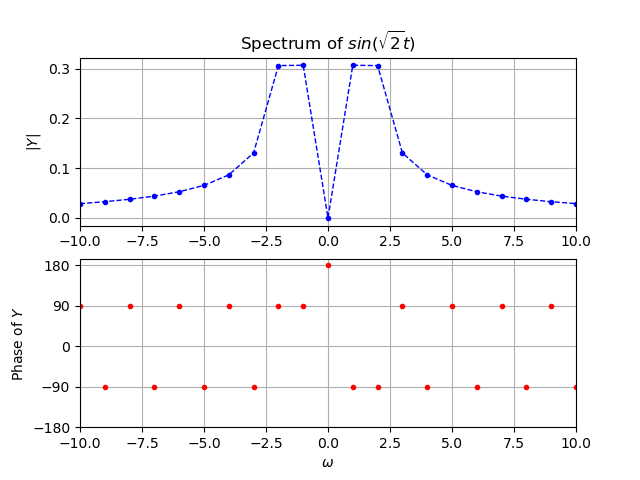
\includegraphics[scale = 0.65]{Figure 0.png}
                \caption{Spectrum of $sin(\sqrt{2}t)$ without windowing}
                \label{fig:Figure 0}
            \end{figure}
        We observe that:
            \begin{enumerate}
            \item We expected two spikes, but what we got were two peaks each with two values and a gradually decaying magnitude.
            \item Since $\sqrt{2} = 1.4142$ is not in the resolution of $\omega$ therefore we get a peak that is two samples wide from $1$ to $2$.
            \item The magnitude is gradually decreasing due the presence of large discontinuities in the $2\pi$ wrapped signal.
            \item The phase is correct.
            \item What went wrong is due to the Gibbs phenomenon. Thus we have a need of windowing the original signal to suppress the discontinuities.
            \end{enumerate}
        \subsubsection{With Hamming window}
        Now we plot the spectrum of the windowed signal, using the Hamming window which is defined in Equation 1. Python code snippet for plotting:
            \begin{verbatim}
Title = r"Spectrum of $sin(\sqrt{2}t)w(t)$"
w,Y = Spectrum(fmax,y,Title,1,[-8,8],True,Yticks=p.arange(0,0.26,0.05))
            \end{verbatim}
            \begin{figure}[!h]
                \centering
                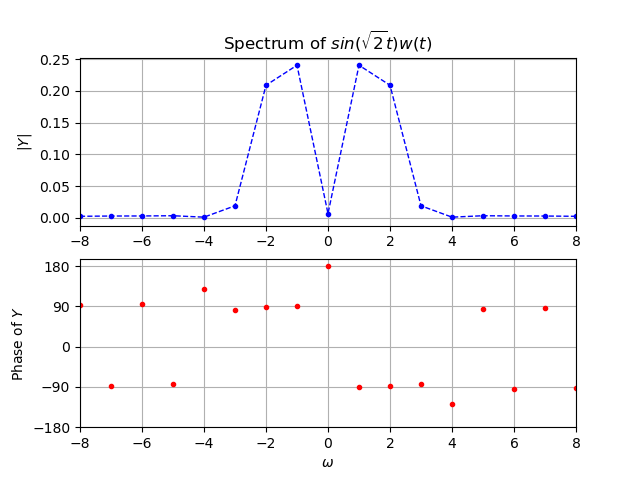
\includegraphics[scale = 0.65]{Figure 1.png}
                \caption{Spectrum of $sin(\sqrt{2}t)w(t)$ with $64$ points}
                \label{fig:Figure 1}
            \end{figure}
        We notice that:
            \begin{enumerate}
            \item The magnitude spectrum has greatly improved.
            \item We still have a peak that is $2$ samples wide, but that is because $\sqrt{2}$ lies between $1$ and $2$, which are the two fourier components available.
            \item If we use four times the number of points i.e. $256$, we should get better results.
            \end{enumerate}
        Using $256$ points in $t = [-4\pi,4\pi)$, thus the fmax remains unchanged. That means the limits of frequency axis remains unchanged. But the number of points in the frequency axis has become four times. Thus resolution increases. Python code snippet:
            \begin{verbatim}
t = p.linspace(-4*pi,4*pi,257)[:-1]
dt = t[1] - t[0];fmax = 1/dt
y = p.sin(p.sqrt(2)*t)
Title = r"Spectrum of $sin(\sqrt{2}t)w(t)$ with four times the number of points"
w,Y = Spectrum(fmax,y,Title,2,[-4,4],True,Yticks=p.arange(0,0.26,0.05))
            \end{verbatim}
            \begin{figure}[!h]
                \centering
                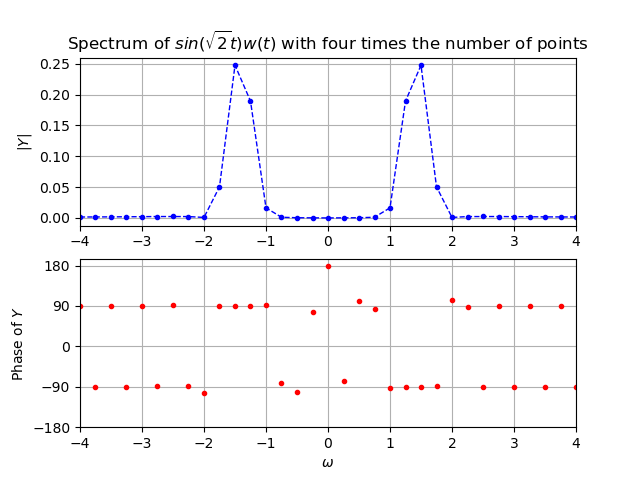
\includegraphics[scale = 0.65]{Figure 2.png}
                \caption{Spectrum of $sin(\sqrt{2}t)w(t)$ with $256$ points}
                \label{fig:Figure 2}
            \end{figure}
        It is quite a bit better since we are now zoomed in and see a lot more
        detail. But again the peak does not look like a delta function and has some width. The reason for that is $w(t)$. Multiplication in time is convolution in frequency and vice versa. So by multiplying with $w(t)$, we got rid of the $1/f$ decay. But the delta function is now replaced by the shape of the DFT of $w[n]$. That gives us a factor of two broadening over the peak when there is no window, which is why we still see a peak whose width is two samples.
    
    \subsection{Spectrum of $cos^3(\omega_0t)$}
        \subsubsection{Without Hamming window}
        First we plot the spectrum without windowing the function with Hamming window. I am using $256$ points on the frequency axis t0 have good resolution. Here $\omega_0 = 0.86$. The python code snippet:
            \begin{verbatim}
y = p.cos(0.86*t)**3
Title = r"Spectrum of $cos^3(\omega_0 t)$"
w,Y = Spectrum(fmax,y,Title,3,[-5,5],Xticks=p.arange(-5,6,1),Yticks = p.arange(0,0.3,0.05))
            \end{verbatim}
            \begin{figure}[!h]
                \centering
                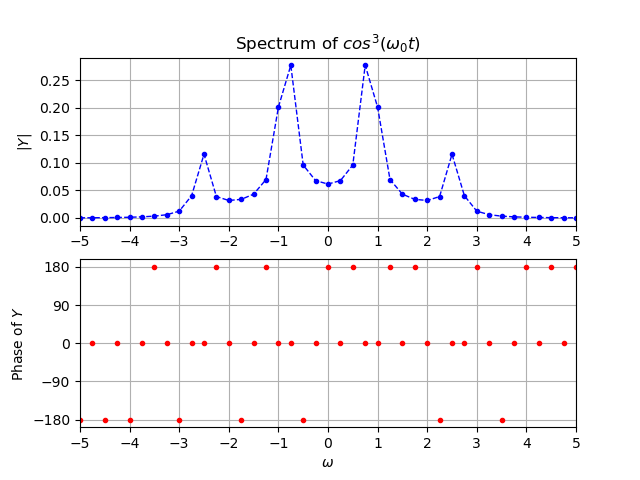
\includegraphics[scale = 0.65]{Figure 3.png}
                \caption{Spectrum of $cos^3(\omega_0 t)w(t)$}
                \label{fig:Figure 3}
            \end{figure}
        We notice:
            \begin{enumerate}
            \item We have four peaks as expected but not exactly where they should have been due to less resoltuion.
            \item Magnitude is \textbf{not} going to zero for frequencies other than peak. This is becauuse we haven't windowed the function.
            \item Phase is correct.
            \end{enumerate}
        \subsubsection{With Hamming window}
        Python code snippet for plotting the spectrum of windowed signal:
            \begin{verbatim}
Title = r"Spectrum of $cos^3(\omega_0 t)w(t)$"
w,Y = Spectrum(fmax,y,Title,4,[-5,5],True,Xticks=p.arange(-5,6,1))
            \end{verbatim}
            \begin{figure}[!h]
                \centering
                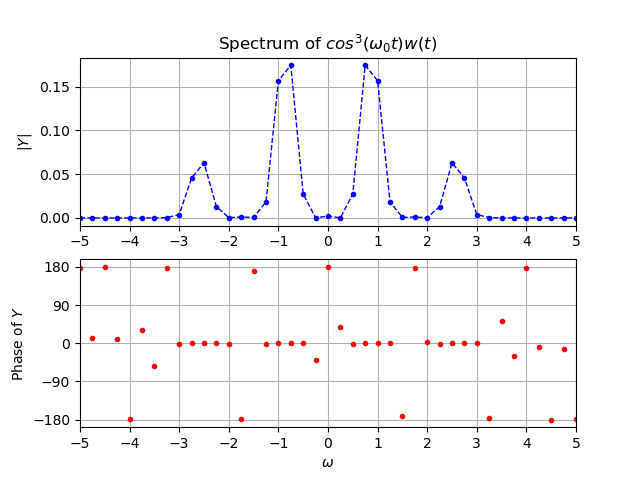
\includegraphics[scale = 0.65]{Figure 4.png}
                \caption{Spectrum of windowed $cos^3(\omega_0 t)$}
                \label{fig:Figure 4}
            \end{figure}
        Magnitude has improved. But still the peaks are not like delta functions but has some width due to reasons mentioned in the previous section.
    
    \subsection{Extracting the spectrum and estimating $\omega_0$ and $\delta$}
    We have a $128$ element vector known to contain $cos(\omega_0 t + \delta)$ for arbitrary $\delta$ and $0.5 < \omega_0 < 1.5$. The values of $t$ go from $-\pi$ to $\pi$. We have to extract the digital spectrum of the signal, find the two peaks at $\pm \omega_0$, and estimate $\omega_0$ and $\delta$.
        \begin{enumerate}
        \item The resolution is not enough to obtain the $\omega_0$ directly. The peak will not be visible clearly because of the fact that resolution of the frequency axis is not enough. So, we have to obtain $\omega_0$ by taking a weighted average of all the $\omega$ weighted with the magnitude of the DFT.
            \begin{equation}
\omega_{cal} = \frac{\sum \omega_i \lvert{Y(\omega_i)}\rvert^2}{\sum \lvert{Y(\omega_i)}\rvert^2} ; \forall \omega_i > 0
            \end{equation}
        \item $\delta$ can be found by calculating the phase of the discrete fourier transform at $\omega$ nearest to estimated $\omega_{cal}$. This works because the phase of $cos(\omega_0 t + \delta)$ when $\delta = 0$ is $0$, so when its not its $\delta$. So we can estimate it by this approach.
        \end{enumerate}
    I have written a function \texttt{w0\_delta()} that takes in as arguments $\omega$ (the frequency axis of transform) and $Y$ (transform), and estimates and prints the values of $\omega$ and $\delta$.
        \begin{verbatim}
def w0_delta(w,Y,prnt=""):
    ii = p.where(w > 0)                                       #Indexes of all w>0
    #Taking weighted average of all w>0 with magnitude of DFT as weights
    w_estimate = sum(w[ii]*abs(Y[ii])**2)/sum(abs(Y[ii])**2)
    #Finding index of nearest w to the estimated w. This is done for finding delta
    i = abs(w - w_estimate).argmin
    #delta(estimated) = angle of Y at the index found above.
    delta_estimate = p.angle(Y[i])
    
    print("\nEstimated w0"+prnt+" = ",w_estimate)      #Printing the estimated w
    print("Estimated delta"+prnt+" = ",delta_estimate) #Printing the estimated
                                                       #delta
        \end{verbatim}
        \subsubsection{Without noise}
        Python code for extracting spectrum:
            \begin{figure}[!h]
                \centering
                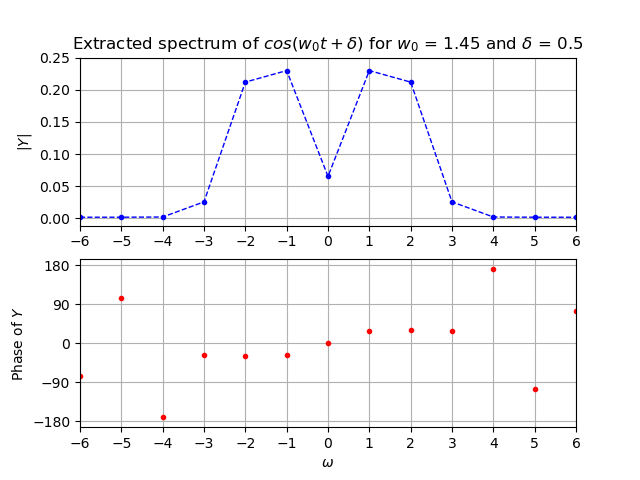
\includegraphics[scale = 0.65]{Figure 5.png}
                \caption{Extracted spectrum of $cos(w_0 t + \delta)$ without noise.}
                \label{fig:Figure 5}
            \end{figure}
            \begin{verbatim}
w0,delta = 1.45,0.5                        #Arbitrary values for w0 and delta
t = p.linspace(-pi,pi,129)[:-1]            #Creating 128 element time axis
dt = t[1] - t[0];fmax = 1/dt
y = p.cos(w0*t + delta)                    #Creating the 128 element vector
Title = r"Extracted spectrum of $cos(w_0 t + \delta)$ for $w_0$ = " + str(w0) + " and 
        $\delta$  = " + str(delta)
w,Y=Spectrum(fmax,y,Title,5,[-6,6],True,Xticks=p.arange(-6,7,1),Yticks=p.arange(0,0.26,0.05))
            \end{verbatim}
        With this we will get $\omega$ and $Y$ which are needed as arguments in the \texttt{w0\_delta()} function to estimate $\omega_0$ and $\delta$. Then to get the estimation of $\omega_0$ and $\delta$ we do \texttt{w0\_delta(w,Y," with noise")}
        The estimated values are (in noiseless case):
            \begin{verbatim}
    Estimated w0 =  1.472374597597627
    Estimated delta =  0.49406546876219665
            \end{verbatim}
        These values are very close to the actual values: $\omega_0 = 1.45$ and $\delta = 0.5$ since there is no noise in the data.
        
        \subsubsection{With noise}
        Python code snippet for extracting the spectrum:
            \begin{verbatim}
y = p.cos(w0*t + delta) + 0.1*p.randn(128)          #Adding noise to the previous
                                                    #vector
Title = r"Extracted spectrum of noisy $cos(w_0 t + \delta)$ for $w_0$ = " + str(w0) + " and 
        $\delta$ = " + str(delta)
w,Y=Spectrum(fmax,y,Title,6,[-6,6],True,Xticks=p.arange(-6,7,1),Yticks=p.arange(0,0.26,0.05))
            \end{verbatim}
            \begin{figure}[!h]
                \centering
                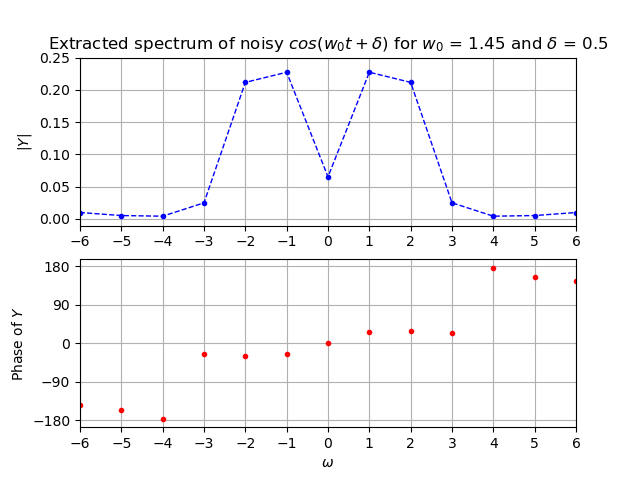
\includegraphics[scale = 0.65]{Figure 6.png}
                \caption{Extracted spectrum of $cos(w_0 t + \delta)$ with noise.}
                \label{fig:Figure 6}
            \end{figure}
        With this we will get $\omega$ and $Y$ which are needed as arguments in the \texttt{w0\_delta()} function to estimate $\omega_0$ and $\delta$. Then to get the estimation of $\omega_0$ and $\delta$ we do \texttt{w0\_delta(w,Y," with noise")}
        \begin{verbatim}
    Estimated w0 with noise =  2.226896537304723
    Estimated delta with noise =  0.5199696772341339
        \end{verbatim}
        These values are not quite close to the actual values as noise is added to the data. The more there is noise, the more difficult it is to extract the peak frequency and phase.
    \subsection{Chirped Signal : $cos(16(1.5 + \frac{t}{2\pi})t)$}
    Python code for plotting the spectrum (using Hamming window). It's given that $t = [-\pi,\pi)$ in 1024 steps.
        \begin{verbatim}
t = p.linspace(-pi,pi,1025)[:-1]        #time axis : 1024 points between [-pi,pi)
dt = t[1] - t[0];fmax = 1/dt
y = p.cos(16*(1.5 + t/(2*pi))*t)
Title = r"Spectrum of $cos(16(1.5 + \frac{t}{2\pi})t)w(t)$"
w,Y = Spectrum(fmax,y,Title,7,[-50,50],True,Xticks = p.arange(-50,51,10))
        \end{verbatim}
        \begin{figure}[!h]
            \centering
            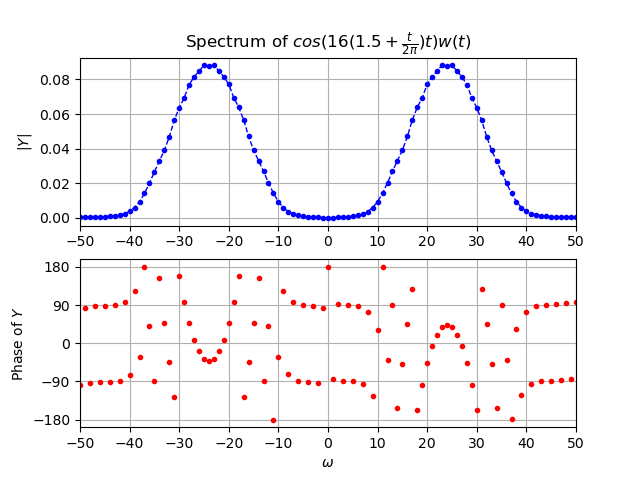
\includegraphics[scale = 0.65]{Figure 7.png}
            \caption{Spectrum of $cos(16(1.5 + \frac{t}{2\pi})t)w(t)$}
            \label{fig:Figure 7}
        \end{figure}
    Its frequency continuously changes from $16$ to $32$ rad/sec. This also means
    that the period is $64$ samples near $-\pi$ and is $32$ samples near $+\pi$. In the plot $w(t)$ is the windowing function.
    
        \subsubsection*{Surface Plot}
        The following code is for making the surface plot to show how the frequency of the signal varies with time.
            \begin{verbatim}
t_array = p.array(p.array_split(t,16))          #Dividing the t array into 16
                                                #sections of 64 elements each
y_array = p.cos(16*(1.5 + t_array/(2*pi))*t_array)   #Calculating and storing the
                                                     #function values at those
                                                     #values of t

n = p.arange(64)
wnd = p.fftshift(0.54 + 0.46*p.cos(2*pi*n/63))
y_array = y_array*wnd                       #Multiplying all 16 sections of y
                                            #with window function
y_array[:,0] = 0        #the sample corresponding to -tmax should be set zero in
                        #all 16 sections
Y_array = p.fftshift(p.fft(y_array))/64     #Calculating the transform

t = t[::64]
w = p.linspace(-pi*fmax,pi*fmax,65)[:-1]
t,w = p.meshgrid(t,w)

#Plotting the surface plot
fig8 = p.figure(8)
ax = fig8.add_subplot(111,projection = '3d')
surf=ax.plot_surface(w,t,abs(Y_array[::-1]).T,cmap='viridis',linewidth=0, antialiased=False)
fig8.colorbar(surf,shrink = 0.5,aspect = 5)
ax.set_title(r"Surface Plot")
p.ylabel(r"$\omega \rightarrow$")
p.xlabel(r"$t \rightarrow$")
p.savefig("Figure 8.png")  #Saving the figure
p.show()
            \end{verbatim}
            \begin{figure}[!h]
                \centering
                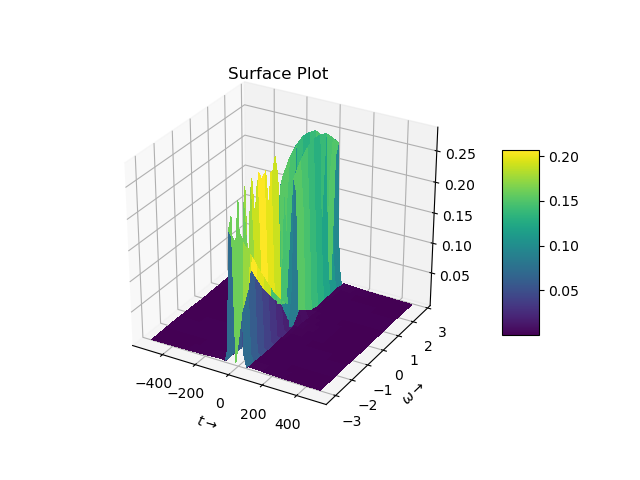
\includegraphics[scale = 1]{Figure 8.png}
                \caption{Surface plot of magnitude}
                \label{fig:Figure 8}
            \end{figure}

\section{Conclusion}
In this assignment:
    \begin{enumerate}
    \item We learnt how to get DFT and plot spectrum of non-periodic functions using windowing.
    \item We learnt about the Hamming window.
    \item We learnt how to estimate the peak frequency and phase from a vector that is known to contain a function value.
    \item We also made a $3$D plot of magnitude of broken Chirped signal
    \end{enumerate}
\end{document}
